\chapter{Implementation}
The scanner has been implemented using the programming language Python, since the language is easier to use than C++ for smaller projects like this one.

\section{Test images}
To test the detection quality of the scanner during implementation already, multiple test images have been taken. They allow to understand how the chosen implementation can handle images taken in different scenarios, like document size and color, lighting conditions or background color. The following images are used:

\begin{itemize}
    \item A4 math sheet on a dark wooden surface (\autoref{fig:overall})
    \\ \textit{easiest to scan because of good contrast}
    \item A4 math sheet on a dark wooden surface, tilted (\autoref{fig:transformation})
    \\ \textit{tests image transformation}
    \item A4 math sheet on a light wooden surface, cut (\autoref{fig:crop})
    \\ \textit{tests corner detection if not all corners are visible}
    \item A4 furniture assembling scheme on a light wooden surface (\autoref{fig:cannymorph}, \autoref{fig:threshold})
    \\ \textit{has worse contrast and crinkles in the paper}
\end{itemize}

The images and their processed versions are used throughout this document to visualize the scanners work.

\section{Used libraries}
For the implementation of the scanner, existing proven libraries have been used to be able to use their features without much additional implementation effort. In Python, packages are most commonly installed using the Python packet manager \enquote{pip} from the Python Package Index (PyPI). To avoid version conflicts of libraries between projects on the computer, a separate virtual environment has also been set up.

Responsible for the main image manipulations is the \enquote{OpenCV} library, which was installed using an unofficial pre-built version as the \texttt{opencv-python} package. \cite{pip_opencv} Additionally, the \enquote{NumPy} package has been installed, which offers a wide variety of mathematical functions and is required for OpenCV. \cite{pip_numpy}

\section{General architecture}
The scanner has been implemented as a separate class \texttt{DocumentScanner} to encapsulate its logic and allow for easy usage in the main function of a program.

The class offers 4 public methods to use:

\subsubsection*{Constructor}
To instantiate the class, three parameters have to be provided to the constructor: the filename of the document, a document format enumeration value and a boolean value whether effects should be applied.

Using the filename, the given image will be loaded into a field so it can be used in all the methods.

The document format must be provided as an enum, which has two options: Auto and A4. The document format can be provided to later allow for an optimal image transformation and output format in \autoref{transf}.

The boolean value indicates whether the black-white effect should be applied to get a binary image as output. As the scanner technically also supports colored documents, this flag offers more flexibility to the user.

\subsubsection*{Scan}
This method contains the main logic to scan the document and returns the requested scanned document. Its implementation is described in \autoref{main_logic}.

\subsubsection*{Save image}
This method allows to save the output from the Scan method in a file. Although this violates the single responsibility principle of object oriented programming, this method has been added for convenience and simplicity to this project. 

\subsubsection*{Show image history}
This method shows the images collected during the intermediate processing steps of the scanning process in a Matplotlib plot. This way, it is easy to understand how the algorithm works visually. Its output images are used throughout this document.

\section{Scanning algorithm}
\label{main_logic}

As described in the last section, the main scanner logic is located in the Scan method. To reduce its complexity, the method has been split in multiple submethods, as seen in \autoref{lst:scan}.

As a reference for this implementation, general ideas from the documentation of \cite{scanner} have been incorporated. Changes have been made whenever it would yield better results, though.

\begin{lstlisting}[caption={Scan method}, label={lst:scan}]
def scan(self):
    img = self.__prepare_image(self.document)
    edged = self.__get_edged_image(img)
    contour = self.__get_best_contour(edged)
    transformed_img = self.__transform_image(self.document, contour)
    if self.apply_effects:
        transformed_img = self.__apply_image_effects(transformed_img)

    return transformed_img
\end{lstlisting}

\subsection{Preparing the image}
\begin{lstlisting}[caption={Prepare image method}, label={lst:prepare}]
IMAGE_HEIGHT = 700
def __prepare_image(self, img):
    # scale down image
    ratio = self.IMAGE_HEIGHT / img.shape[0]
    img = cv2.resize(img, (int(ratio * img.shape[1]), self.IMAGE_HEIGHT))

    # gaussian blur to reduce noise
    img = cv2.GaussianBlur(img, (5, 5), 0)
    return img
\end{lstlisting}
    
To start the scanning process, in \autoref{lst:prepare} the loaded image will be downscaled to 700 pixels height to reduce computational effort and unnecessary information in the image. The same applies to the use of the gaussian blur afterwards, so later only strong edges are detected.

Now the image could be converted to grayscale to further reduce its complexity. In the following implementation, this won't be done though. Firstly because all OpenCV functions used also accept a colored image, but mainly because in testing this yielded better results in the edge detection for all test images. Since the edge detector internally also has to convert the image to grayscale, possibly the edge detector uses a more optimized grayscale conversion algorithm than is provided with the default \texttt{cvtColor} (\texttt{COLOR\_BGR2GRAY}) implementation of OpenCV.

\subsection{Edge detection}

After the image has been prepared, now the edges in the image have to be detected to find the document. For this, the Canny edge detector provided by OpenCV is used. It was first described by John Canny in 1986 \cite{canny_paper} and is since then used as a proven edge detector, and is easy to use in OpenCV. It calculates the intensity gradient of the image, then performs non-maximum suppression and finally chooses the most promising edges with hysteresis thresholding, as firmly described in \cite{cv_canny}.

\begin{lstlisting}[caption={Edge detection method}, label={lst:edge}]
def __get_edged_image(self, img):
    # run canny edge detector
    edged = cv2.Canny(img, 70, 120)

    # connect lines that may be disconnected a bit
    kernel = np.ones((5, 5), np.uint8)
    edged = cv2.morphologyEx(edged, cv2.MORPH_CLOSE, kernel)

    return edged
\end{lstlisting}

As seen in \autoref{lst:edge}, the OpenCV implementation takes the image and a lower and upper threshold as parameters. The image used can be colored, as described earlier.

For the determination of the thresholds, multiple combinations with values between 0 and 255 (8 byte color value) and the result of its Canny edged image were checked.

First, a simple automatic threshold selection algorithm has been tested for grayscale images, as described in \cite{autocanny}. It calculates the median (or mean) value of the image and sets the lower threshold to be $1/3$ lower than the median/mean, and the higher threshold $1/3$ higher than the median/mean. Because large parts of the image are white though, this would create an unwanted bias to lower values and therefore result in worse edge detection for the test images. Hence this approach was not further examined and fixed thresholds were used instead.

The contrast or rather gradient between a white document, its shadow and the table surface across the entire edge can differ because of lighting conditions, paper crinkles and image perspective. Therefore the lower threshold couldn't be set too high - otherwise small badly lighted parts of the edge could result in the entire edge to be discarded. 70 has been found as a good compromise value for the testing images.

Due to the same reason, the higher threshold couldn't be too high as well, otherwise possibly no relevant edges at all would be detected. Setting a lower value is not a problem though, since the table usually has a smooth surface without edges, making the document easily identifiable. Thus 120 has been selected for this implementation after experimenting with the test images.

The Canny edge detector now returns a binary image containing the detected edges. When inspected, especially using the crinkled assembly document, the edge wasn't identified across the entire contour of the paper and had small disconnected \enquote{holes}. This can be seen circled red in \autoref{fig:cannymorph} where there is a small hole in the contour, making it not closed.

To solve this issue, the edged image is run through the \texttt{morphologyEx} function of OpenCV with the \texttt{MORPH\_CLOSE} parameter. It can close small holes in lines, effectively merging edges that are close to each other, as seen in \autoref{fig:cannymorph}. The kernel parameter determines how big the local neighborhood to be inspected should be. With this step, the edge is detected as continuos. More implementation details can be found in \cite{cv_morph}.

\begin{figure}[h]
    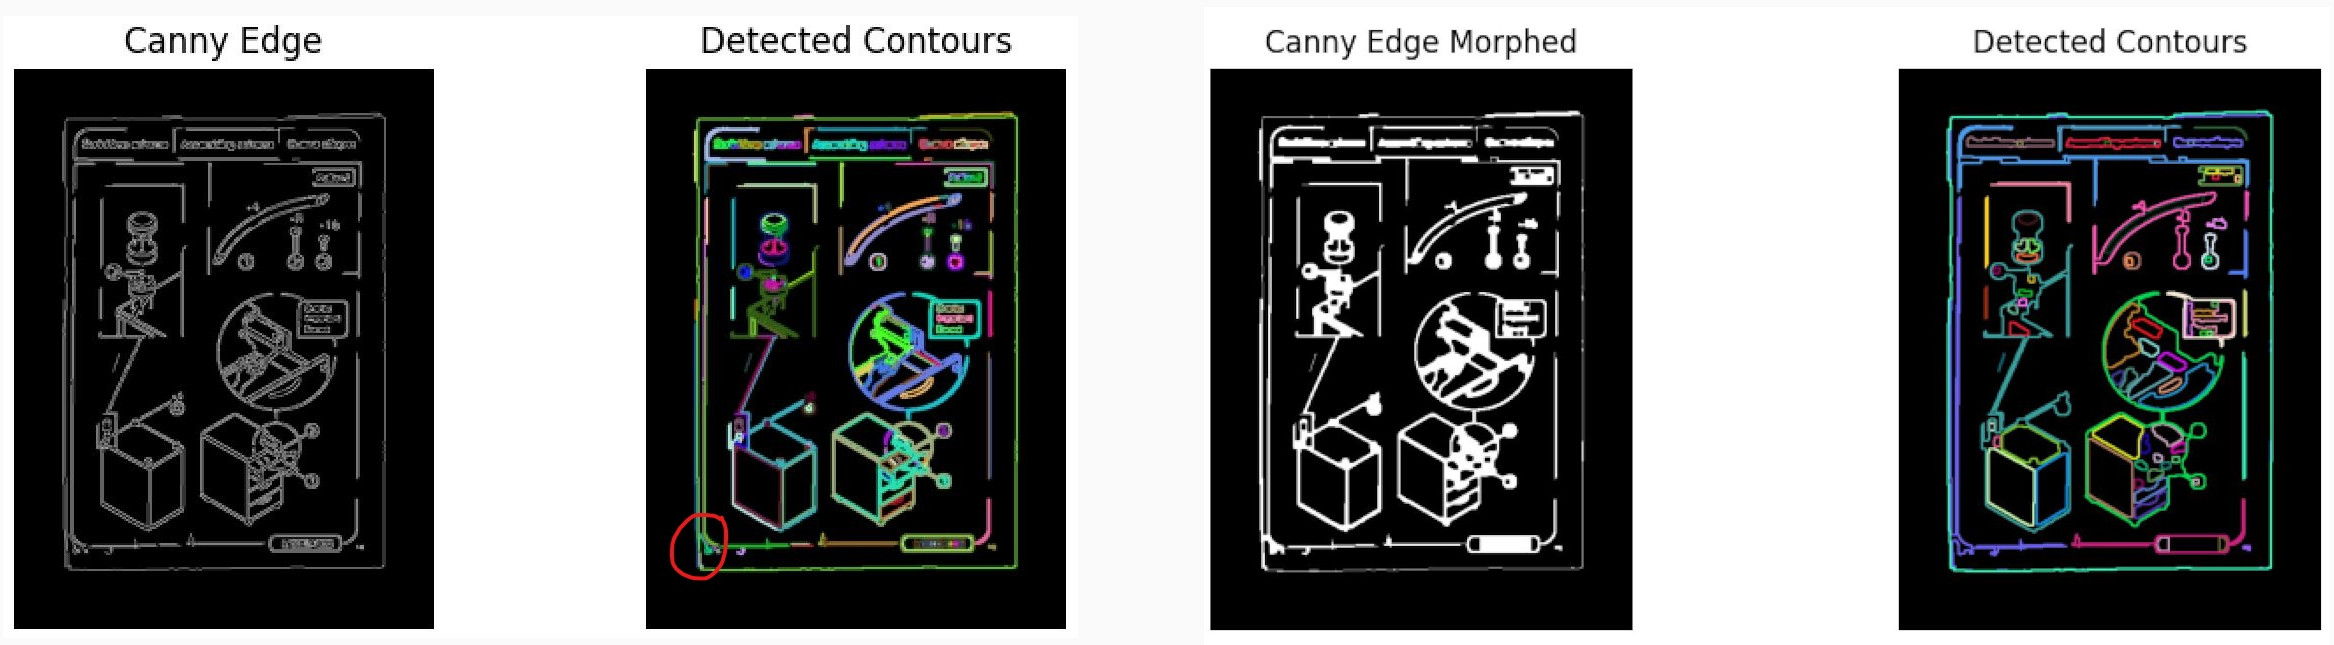
\includegraphics[width=1\textwidth]{figures/canny.jpg}
    \centering
    \caption{Closed contour by using morphing of Canny edged image}
    \label{fig:cannymorph}
\end{figure}

\subsection{Identifying document contour}

\begin{lstlisting}[caption={Contour detection method}, label={lst:contour}, float]
def __get_best_contour(self, edged_img):
    # get contours
    contours, _ = cv2.findContours(edged_img, cv2.RETR_LIST, cv2.CHAIN_APPROX_SIMPLE)

    # calculate contour area
    contour_areas = map(cv2.contourArea, contours)
    contours_with_areas = zip(contours, contour_areas)

    # contour must span at least 40% of image area
    img_height, img_width = edged_img.shape
    min_area = img_height * img_width * 0.4
    filtered_contours = filter(lambda tup: tup[1] >= min_area, contours_with_areas)

    # sort remaining contours by the area they span
    sorted_contours = sorted(filtered_contours, key=lambda tup: tup[1], reverse=True)

    for contour, _ in sorted_contours:
        # approximate the contour as rectangle
        eps = 0.05 * cv2.arcLength(contour, True)
        approx = cv2.approxPolyDP(contour, eps, True)
        # use first (biggest) contour that has 4 corners as our best contour
        if len(approx) == 4:
            return approx

    # if no fitting contour was found, return contour of entire image
    return np.array([[[0, 0]], [[0, img_height]], [[img_width, img_height]], [[img_width, 0]]])
\end{lstlisting}

With a set of edges found in the image by the Canny edge detector, now the actual document contour must be found, as seen in \autoref{lst:contour}.

OpenCV offers the \texttt{findContours} function to do this, using the edged image returned by the Canny edge detector. A contour is identified as a set of points found on a continuos line or curve. The \texttt{CHAIN\_APPROX\_SIMPLE} flag simplifies the contours found by reducing the points needed to describe the contour, making computations easier. Since the hierarchy of contours is not required for this application, the flag \texttt{RETR\_LIST} is used here.

The now returned contours are described by actual coordinates, making further calculations possible. First, the area of all contour shapes is calculated. Optimally, the document can be identified by the contour with the biggest contour area. Thus smaller contours, for example text or graphics in the document, can be filtered out by setting an area threshold. Here, the assumption has been made that the document must fill at least 40\% of the entire image area. This value could be adapted for different document sizes however.

Now having a even more reduced set of contour candidates, more detailed calculations can be done. For this, in a loop the remaining contours are simplified even more using the \texttt{approxPolyDP} function, which uses the \enquote{Ramer-Douglas-Peucker} algorithm. The epsilon value identifies the maximum distance between the original curve and its approximation, for which reason a value proportional to the perimeter of the contour is used. \cite{cv_approx}

The now calculated, simplified contours should only have as many points as needed to describe the shape of the contour. Since luckily a document generally has exactly 4 edges, contours that have more or less contours can be filtered out as well. Because the list of contours was sorted by area before, the first matching contour is now identified as the document contour and returned as the \enquote{best} contour. The contour is identified by exactly 4 corner points of the document.

In case no contour can be found, the function returns the contour of the complete input image to avoid unexpected behavior in the further processing. This can happen if for example the gradient between the document and background surface isn't big enough, the 4 edges of the document are not completely visible in the image or there actually is no document on the image. An example for this can be seen in \autoref{fig:crop}, where the final contour found is the image itself (seen with the green outline on the right image).

\begin{figure}[h]
    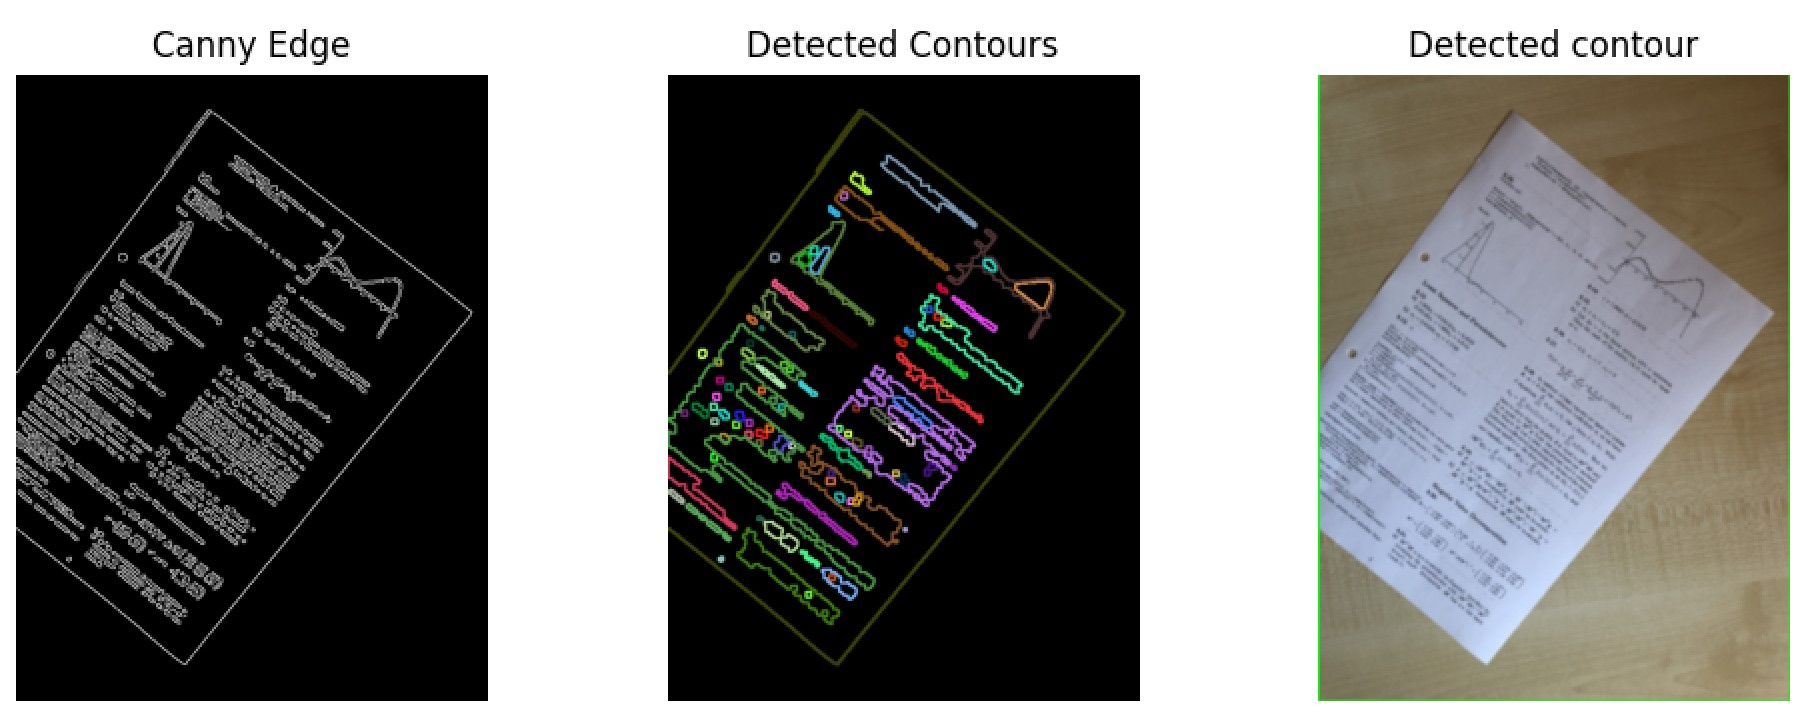
\includegraphics[width=0.8\textwidth]{figures/cut.jpg}
    \centering
    \caption{Failed contour recognition}
    \label{fig:crop}
\end{figure}

\subsection{Perspective transformation}
\label{transf}

\begin{lstlisting}[caption={Image transformation method}, label={lst:transform}, float]
def __transform_image(self, img, contour):
    contour_pts = self.__order_points_clockwise(contour.reshape(4, 2))
    scale = img.shape[0] / self.IMAGE_HEIGHT
    src_pts = (contour_pts * scale).astype(np.float32)

    width = max(np.linalg.norm(src_pts[3] - src_pts[2]),
                np.linalg.norm(src_pts[1] - src_pts[0]))

    if self.format == DocumentFormat.A4:
        height = width * np.sqrt(2)
    else:
        height = max(np.linalg.norm(src_pts[3] - src_pts[0]),
                        np.linalg.norm(src_pts[2] - src_pts[1]))

    dst_pts = np.array([[0, 0],
                        [width, 0],
                        [width, height],
                        [0, height]],
                        dtype=np.float32)

    M = cv2.getPerspectiveTransform(src_pts, dst_pts)
    return cv2.warpPerspective(img, M, (int(width), int(height)))
\end{lstlisting}

After having found the corners of the document, the original image can be cropped and transformed to the found points so only the document is visible, without any background.

First in \autoref{lst:transform}, the corners of the document need to be sorted following some convention (here clockwise) so the transformation is always correct. Also, the point coordinates need to be scaled up again to the original image size.

To calculate the actual width of the new document, the longest distance between the opposite upper and lower points on the left and right are calculated using the 2-norm (euclidean distance). The bigger value is then used.

If the user has specified they were scanning a A4 (or any other DIN normed) document, the height can now be calculated directly by multiplying with the factor $\sqrt{2}$ - since the format of the document is standardized. If the user selected the automatic document size detection, the height will be calculated analogous to the width.

The problem with the latter approach is that the ratio of the width and height may not match the actual ratio of the paper document. This especially happens if the image taken has a tilted perspective. By calculating the height with the primary approach, the ratio information can be obtained regardless of image tilt and the output image will have the correct ratio, too.

To detect documents of other sizes, either more ratio preselections have to be implemented in the algorithm, or the user should take the images without any tilt so they can rely on the automatic calculation. More advanced algorithms detecting the homography could be used as well, but are generally not necessary for this application.

\begin{figure}[h]
    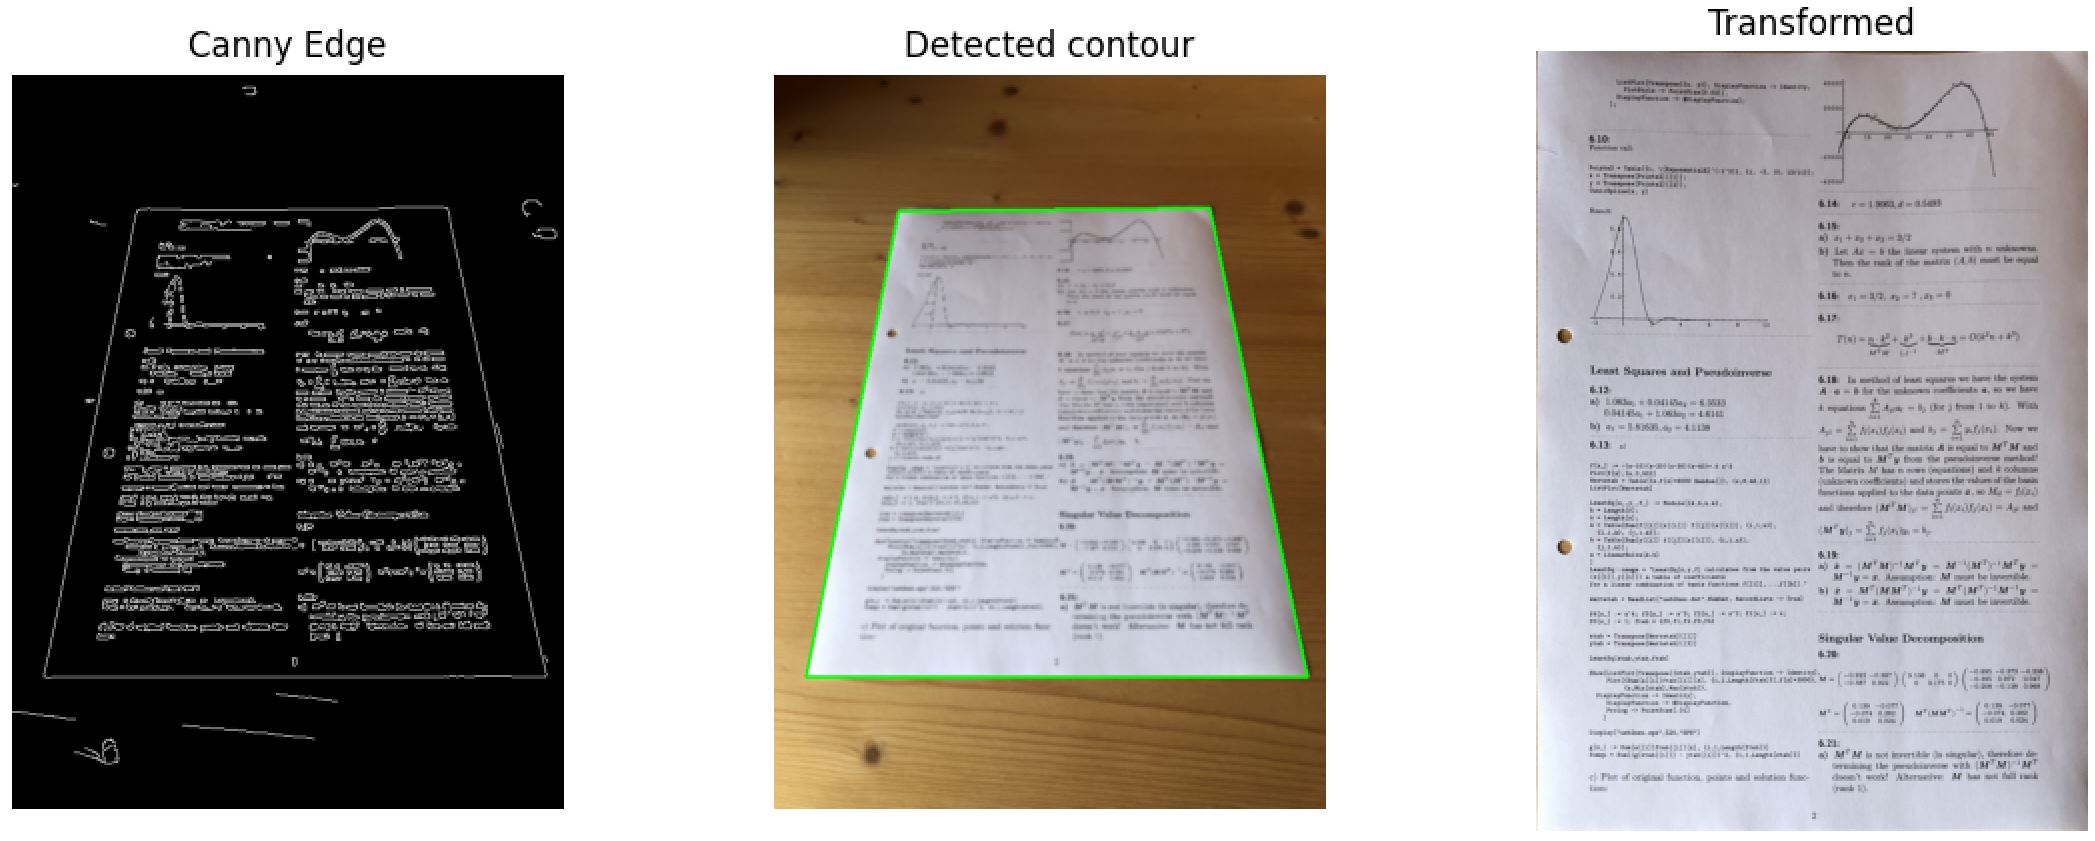
\includegraphics[width=0.8\textwidth]{figures/transformation_tilt.jpg}
    \centering
    \caption{Successful image transformation}
    \label{fig:transformation}
\end{figure}

Finally, to execute the transformation, a transformation matrix needs to be set up that transforms the source points to the destination points - former being the document corners and latter the new full image dimensions.

OpenCV offers the \texttt{getPerspectiveTransform} function to do this without any mathematical knowledge needed. The \texttt{warpPerspective} function then multiplies this matrix with the image to perform the transformation returning the cropped and transformed image. The result of the transformation for a tilted image of a document using the \enquote{A4 setting} can be seen in \autoref{fig:transformation}.

\subsection{Binary image conversion}
\begin{lstlisting}[caption={Image effects method}, label={lst:effects}, float]
def __apply_image_effects(self, img):
    img_gray = cv2.cvtColor(img, cv2.COLOR_BGR2GRAY)
    return cv2.adaptiveThreshold(img_gray, 255, cv2.ADAPTIVE_THRESH_GAUSSIAN_C, cv2.THRESH_BINARY, 11, 15)
\end{lstlisting}

After having created the transformed image, as a final step in \autoref{lst:effects} the binary black-and-white \enquote{scanned} effect needs to be added to the image (if the user requested this).

First, the image must first be converted to grayscale - reducing the three color channels to just a single one. The \texttt{cvtColor} function of OpenCV is capable of doing this with the flag \texttt{COLOR\_BGR2GRAY} since the initial image was loaded without any additional flags (so in the \textbf{B}lue\textbf{G}reen\textbf{R}ed format).

The grayscale image now has 256 different brightness levels for each pixel. To get the clean scanned look, the image should only have two brightness levels for each pixel - black and white. Therefore, a threshold needs to be set at which it is decided whether a pixel will become black or white.

The simplest approach would be to set a fixed value in between 0 and 255 - for example 128. But as the task \cite{cv_lecture_ex} states, this approach is not sufficient for this application, reason being the uneven lighting conditions when taking the image. When in reality the paper always has the same white color, on the image there may be different levels of brightness due to the direction of (sun)light or unwanted shadows in paper crinkles. These can result in big parts of the image then becoming completely black, just because they were in the shadow.

A better approach is to have an adaptive threshold that changes across the image. The OpenCV function \texttt{adaptiveThreshold} checks the neighborhood of each pixel and takes them into account to calculate a threshold for each pixel. The neighborhood threshold value can be calculated using a simple mean or a bit more advanced weighted mean with respect to the gaussian distribution. Since this application isn't performance critical, the \texttt{ADAPTIVE\_THRESH\_GAUSSIAN\_C} can be chosen, subjectively delivering slightly better results when testing on the images.

Comparing it to the fixed threshold in \autoref{fig:threshold}, the adaptive threshold is clearly better - the shadows on the sheet of paper are completely black with the fixed value, while the adaptive threshold has no problem.

\begin{figure}[h]
    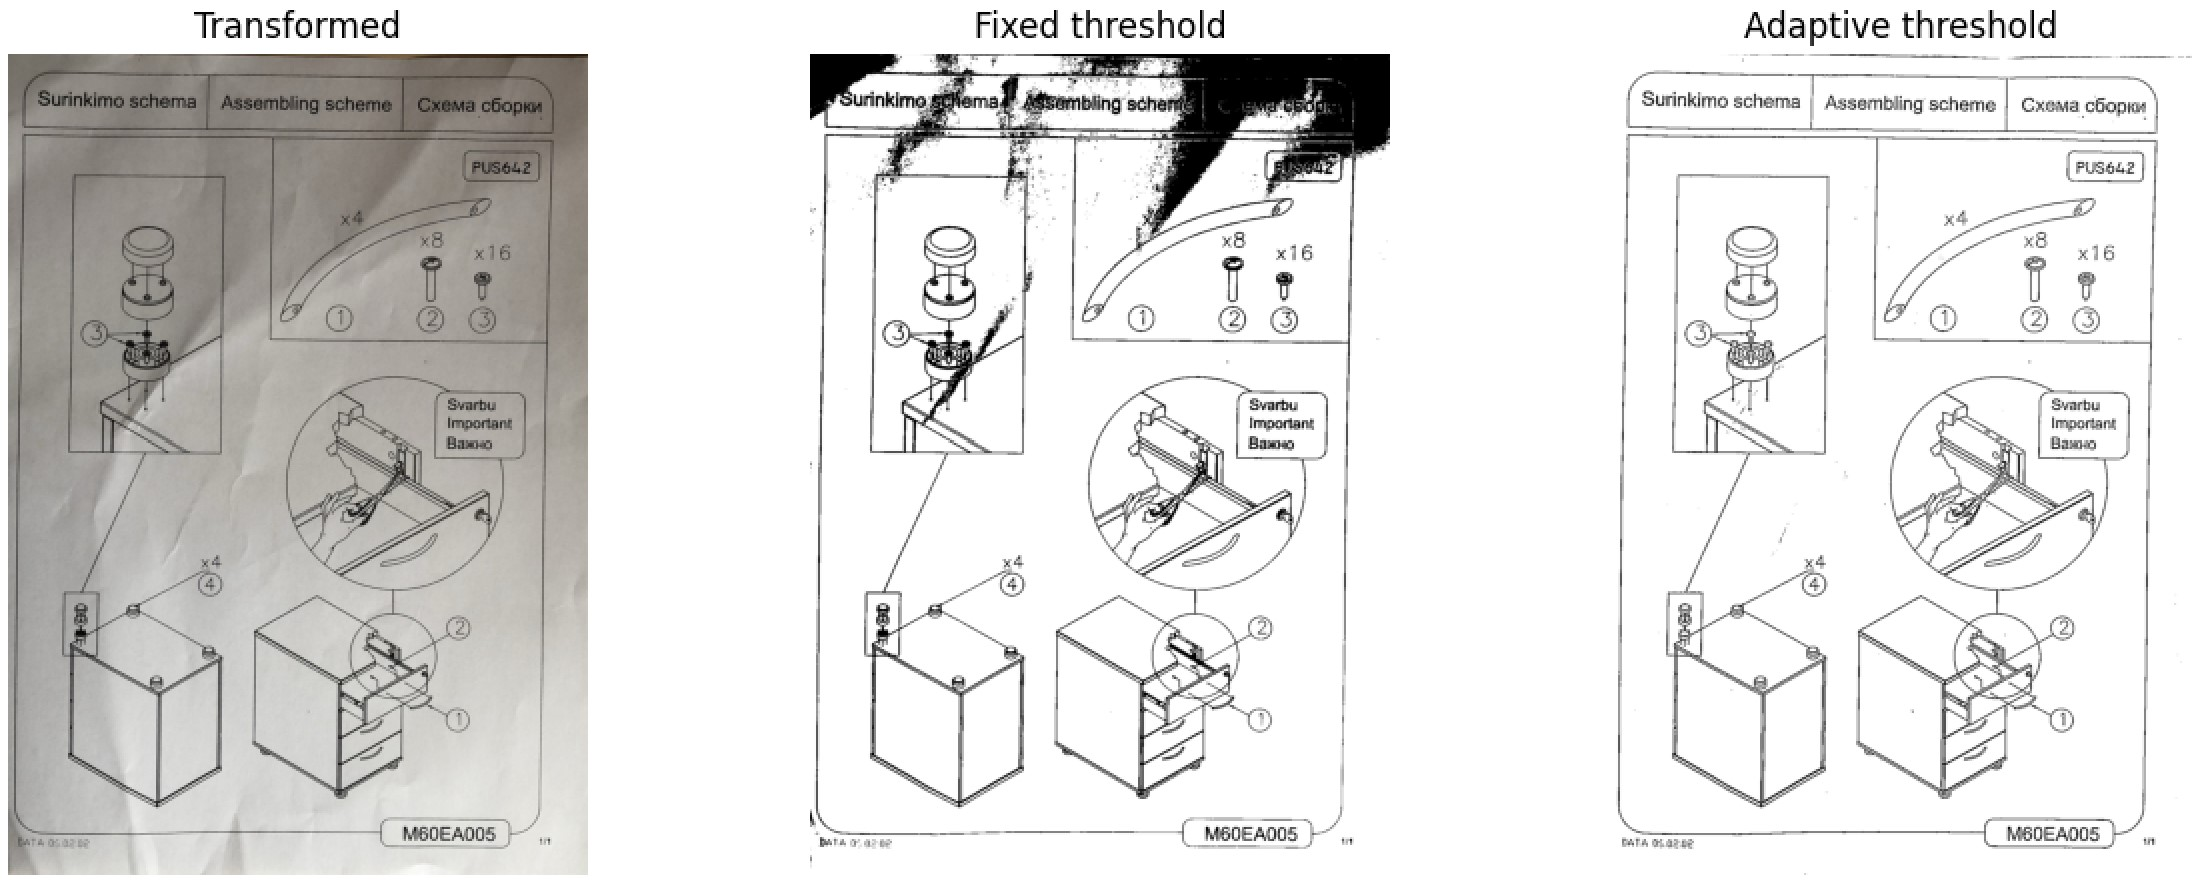
\includegraphics[width=0.8\textwidth]{figures/fixed_thr.jpg}
    \centering
    \caption{Comparison of fixed and adaptive threshold}
    \label{fig:threshold}
\end{figure}